% !TeX root = ../sdc_regulations.tex

\section{Competition Rules}

\subsection{Playing Field}
The playing field is a rectangular area with the following dimensions (Figure 2) :
\begin{itemize}
	\item{Length: 20 meters}
	\item{Width: 10 meters}
	\item{Height: 6 meters}
\end{itemize}

% Abbildung der Ziel-Box (innerhalb der Section)
The playing field is divided into three zones:
\begin{itemize}
	\item{Two Team Zones (red and blue): The home base of each team, where the drones start, land and targets are strategically located.}
	\item{One Neutral Zone in the middle: A neutral territory for strategic maneuvers.}
\end{itemize}
The sizes shown in the graphic are approximate values. The exact dimensions may vary slightly.

\begin{figure}[H]
\centering
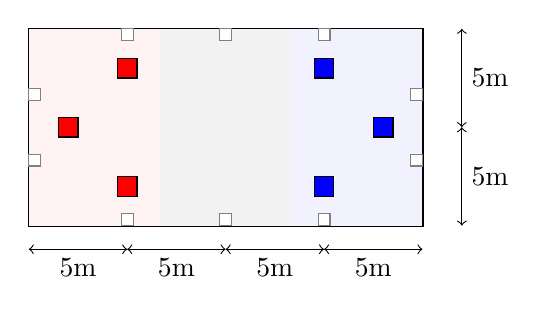
\begin{tikzpicture}[scale=0.25]
	% Maße (m)
	\def\L{20}   % Länge (x)
	\def\W{10}   % Breite (y)

	% Hilfswerte: 3 gleich große Zonen entlang X
	\def\xA{6.67}
	\def\xB{13.33}

	% Rahmen
	\draw[thick] (0,0) rectangle (\L,\W);

	% Sektionen entlang der x-Achse
	\draw[dashed,red!70]  (\xA,0) -- (\xA,\W);
	\draw[dashed,blue!70] (\xB,0) -- (\xB,\W);

	% Sektionen entlang der y-Achse (3 gleich große à ~3.33 m)
	\draw[dashed,gray!70] (0,0.5) -- (\L,0.5);

	% Farbige Zonen
	\fill[red!5]   (0,0) rectangle (\xA,\W);
	\fill[gray!10] (\xA,0) rectangle (\xB,\W);
	\fill[blue!5]  (\xB,0) rectangle (\L,\W);

	% Rand-Boxen (oben/unten): jetzt bei x = 5,10,15 (20 wäre Ecke)
	\foreach \x in {5,10,15}{
	\draw[draw=gray,fill=white] (\x-0.3,0) rectangle ++(0.6,0.6);
	\draw[draw=gray,fill=white] (\x-0.3,\W-0.6) rectangle ++(0.6,0.6);
	}

	% Rand-Boxen (links/rechts) unverändert
	\foreach \y in {3.33,6.66}{
	\draw[draw=gray,fill=white] (0,\y-0.3) rectangle ++(0.6,0.6);
	\draw[draw=gray,fill=white] (\L-0.6,\y-0.3) rectangle ++(0.6,0.6);
	}


	% Beispiel-Targets (weiße Quadrate)
	% Linke drei Boxen rot
	\foreach \x/\y in {5/2, 2/5, 5/8}{
	\draw[fill=red] (\x-0.5,\y-0.5) rectangle ++(1,1);
	}
	% Rechte drei Boxen blau (alle im blauen Segment > 16.66)
	\foreach \x/\y in {15/2, 18/5, 15/8}{
	\draw[fill=blue] (\x-0.5,\y-0.5) rectangle ++(1,1);
	}



	% Maßpfeile X-Achse (in 5m-Sektionen): 0–5,5–10,10–15,15–20
	\foreach \x in {0,5,10,15}{
	\draw[<->] (\x,-1.2) -- (\x+5,-1.2) node[midway,below]{\SI{5}{m}};
	}

	% Maßpfeile Y-Achse (je ~5.0 m)
	\foreach \ya/\yb in {0/5.0,5.0/10}{
	\draw[<->] (\L+2,\ya) -- (\L+2,\yb) node[midway,right]{\SI{5}{m}};
	}

\end{tikzpicture}
\caption{Field Dimensions}
\label{fig:playing-field}
\end{figure}

\subsection{Target Objects}
The objective of the game is to change the color of the target objects to your team's color (red or blue). All gameplay mechanics, scoring rules, and special conditions are described in detail in Section~\ref{sec:game-logic}.
\begin{itemize}
	\item{Each team zone has three target objects, for a total of 6 in the playing field.}
	\item{These objects change their color based on their interaction with the drones:}
	\begin{itemize}
		\item{Default state: Matches the color of the team zone.}
		\item{Triggered state: When an enemy drone approaches and targets the box, it changes to the attacking team's color, updates the ArUco marker, and plays a horn signal. A subsequent enemy drone from the opposing team can then trigger it again.}
	\end{itemize}
	\item{Dimensions of each target box:}
	\begin{itemize}
		\item{Height: \SI{55}{\centi\meter} (open: \SI{73}{\centi\meter}), Width: \SI{57.5}{\centi\meter}, Depth: \SI{37.5}{\centi\meter}}
	\end{itemize}
	\item{Detection: The target boxes detect approaching drones via an internal NFT tag attached to the drone. The system can reliably identify drones within a height range of approximately 1--2 meters. Further specifications and details will be provided in an upcoming update.}
\begin{figure}[h]
\centering
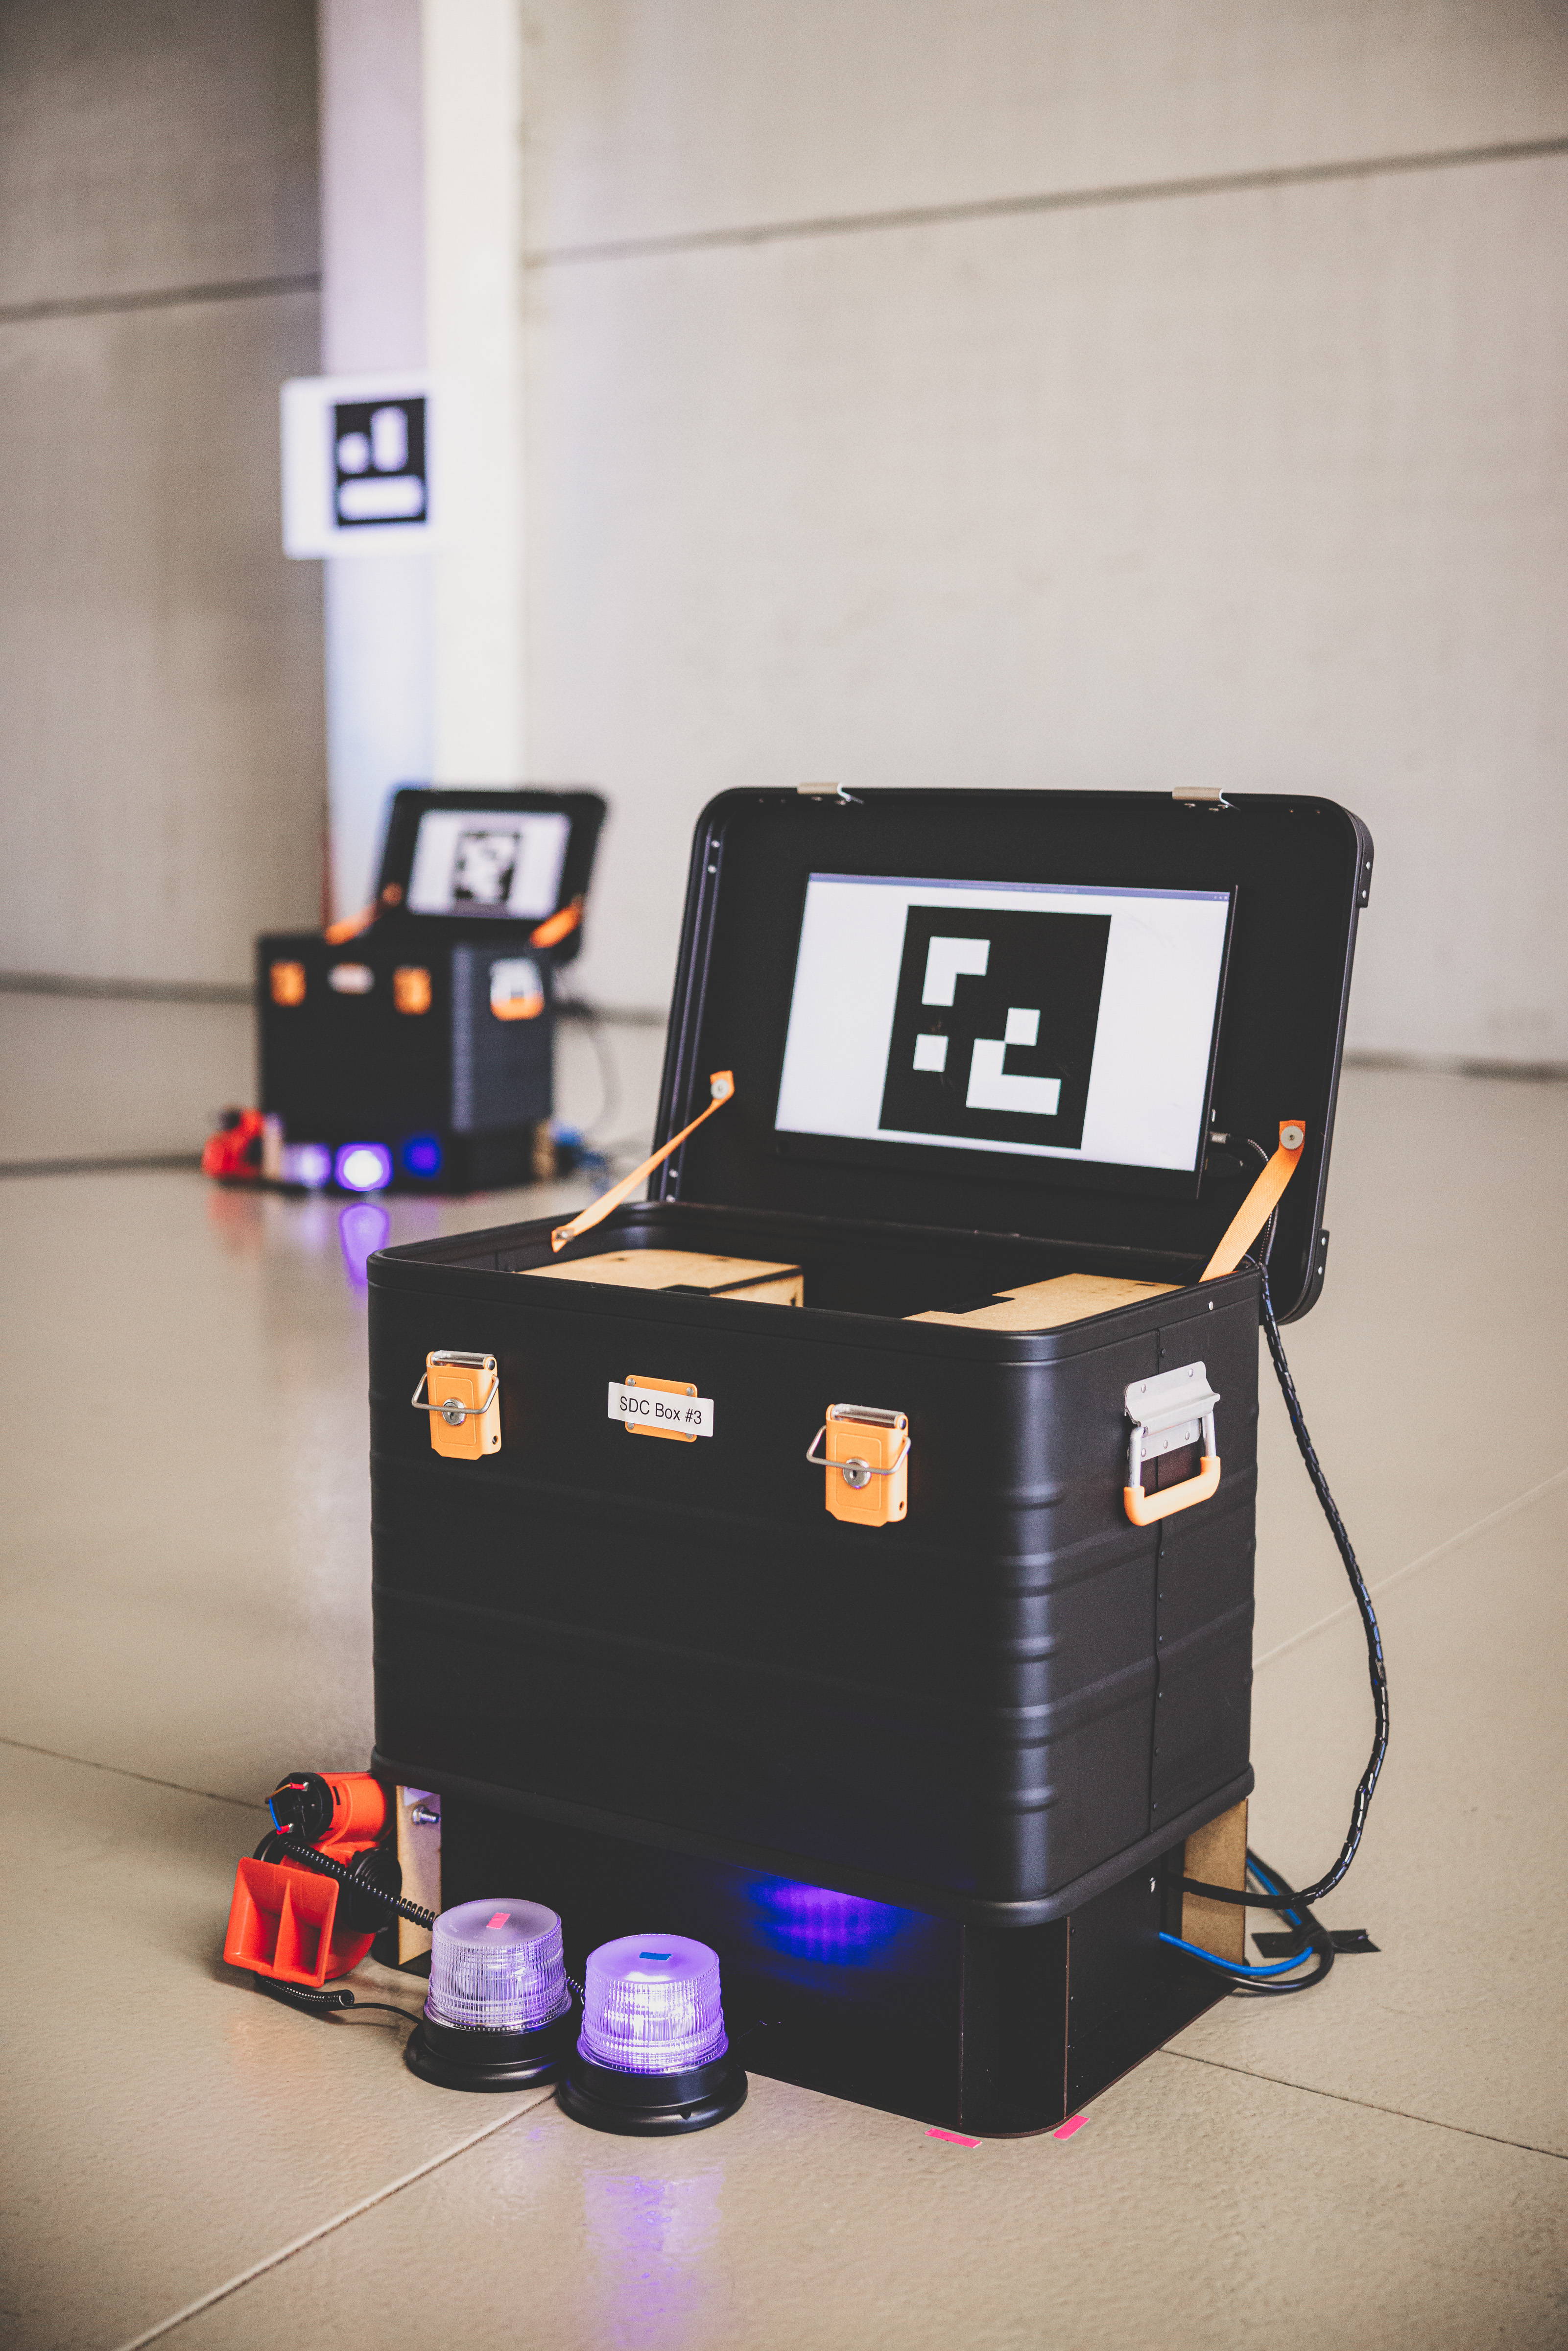
\includegraphics[width=0.2\linewidth]{figures/brigk_SDC2024_206_R5P_0121.jpg}
\caption{Example of an SDC target box.}
\label{fig:target-box}
\end{figure}
\end{itemize}

\subsection{Gameplay}
\label{sec:gameplay}
\begin{itemize}
	\item{Teams: 2--5 drones per team (independent team sizes), ready to battle!}
	\item{Start Setup: Drones may be placed inside their designated team zone and powered on within the cage.}
	\item{Cage Clearance: Once all human operators and staff have exited the cage and the area is confirmed clear, the cage is closed.}
	\item{Final Start Signal: After the cage is secured, the final start signal is given and all drones are permitted to take off and begin flight operations.}
	\item{Action: Drones fly around the arena, trigger target objects to change color, and score points for their team. Full scoring rules are defined in Section~\ref{sec:game-logic}.}
	\item{Target Configuration: The positioning of the target objects within the arena will vary for each match. This ensures that teams cannot pre-program their drones for fixed setups and must rely on real-time perception, adaptability, and autonomous decision-making during gameplay.}
	\item{Defense Strategy:
	Teams may defend target boxes by positioning drones nearby.
	Strictly prohibited: physical obstruction, continuous hovering over targets, capture system interference, and all forms of \textbf{jamming or electronic warfare}.
	\textbf{"Sitting dead duck" behavior} — that is, passive sitting or hovering directly above the boxes — is not allowed and will lead to \textbf{disqualification}.}
	\item{Time Limit: The game lasts for a maximum of 10 minutes. The team with the most points at the end wins the game!}
\end{itemize}

% ── REMOVED RULES (red) — superseded by Game Logic section ──────────────────
\color{red}
\subsubsection[Scoring (removed)]{\textcolor{red}{Scoring (removed --- see Game Logic)}}

\begin{itemize}[label=--]

\item{Scoring Methods:
	\begin{itemize}
		\item Standard Capture (1 Point): Drone captures target box, holds for validation time, returns to home zone before re-capture.
		\item Special Capture (5 Points): Single drone captures box, entire team returns to home base together.
		\item Simultaneous Capture (10 Points): Multiple drones capture boxes at the same time.
	\end{itemize}
}

\item{Capture Stability:
A target box must remain in the capturing team's color for at least \textbf{5 seconds} to validate capture.
Own drone must hover over box for \textbf{2 seconds} to revert color change.
Instant/rapid changes do not count.}

\item{Home Zone Validation:
The drone or drone team must enter the home zone completely and remain inside for at least \textbf{5 seconds}.
Brief or partial contact with the home zone does not validate a capture.}

\item{Simultaneous Capture:
Bonus points are awarded only when two or more \textbf{different target boxes} are captured by different drones of the same team \textbf{simultaneously}.}

\item{Special Maneuver:
When all six target objects display the same team color continuously for at least \textbf{5 seconds}, the team wins the game instantly.
Temporary or unstable color states do not trigger a victory.}

\end{itemize}
\color{black}

% ── NEW SECTION (green) ──────────────────────────────────────────────────────
\color{green!60!black}
\subsection[Game Logic]{\textcolor{green!60!black}{Game Logic}}
\label{sec:game-logic}

\subsubsection[Goal]{\textcolor{green!60!black}{Goal}}
Score points by conquering enemy boxes and finish the match with more points than the other team, or win instantly with a Special Maneuver.

\begin{itemize}
	\item{A team may play with any number of drones.}
	\item{\texttt{5-point} and \texttt{10-point} captures are only possible if the team started the game with at least \texttt{2} drones.}
	\item{With fewer than \texttt{2} drones, only \texttt{1-point} captures and the Special Maneuver are possible.}
\end{itemize}

\subsubsection[ArUco Marker Encoding]{\textcolor{green!60!black}{ArUco Marker Encoding}}
Each physical box displays an ArUco marker from the \texttt{DICT\_4X4\_50} dictionary. The marker ID encodes the current state of the box:
\begin{itemize}
	\item{\texttt{4x} — box is currently \textbf{red}.}
	\item{\texttt{3x} — box is currently \textbf{blue}.}
	\item{The second digit is the \textbf{box ID} (1--6).}
\end{itemize}

\begin{table}[H]
\centering
\begin{tabular}{ccc}
\hline
\textbf{Box ID} & \textbf{Color} & \textbf{Marker ID} \\
\hline
1 & red  & 41 \\
2 & red  & 42 \\
3 & red  & 43 \\
4 & blue & 34 \\
5 & blue & 35 \\
6 & blue & 36 \\
\hline
\end{tabular}
\caption{Default ArUco marker IDs per box (match start).}
\label{tab:aruco-ids}
\end{table}

When a box is captured, the displayed marker changes with the box color. Example: box \texttt{3} starts red (marker \texttt{43}), is captured by blue (changes to \texttt{33}), then recaptured by red (changes back to \texttt{43}).

\subsubsection[Capturing a Box]{\textcolor{green!60!black}{Capturing a Box}}
An enemy box changes to your team's color if:
\begin{itemize}
	\item{your drone hovers over it for at least \texttt{2 seconds}, and}
	\item{no defending drone is detected in that box.}
\end{itemize}

A home-zone box changes back to your team's color immediately when recaptured.

After a successful capture, the box is locked for \texttt{5 seconds}.

\paragraph{\textcolor{green!60!black}{1 Point}}
You get \texttt{1 point} if:
\begin{itemize}
	\item{your team captures an enemy box,}
	\item{the capturing drone returns home, and}
	\item{this happens before that box is recaptured by the other team.}
\end{itemize}

If the box is recaptured first, you still get \texttt{1 point} only if the capturing drone had already reached home; otherwise you get \texttt{0}.

\paragraph{\textcolor{green!60!black}{5 Points}}
You get \texttt{5 points} if:
\begin{itemize}
	\item{your team captures an enemy box,}
	\item{your team started the game with at least \texttt{2} drones,}
	\item{at the moment of capture, all drones of your team are \textbf{outside} your home zone, and}
	\item{then all your drones return home before that box is recaptured.}
\end{itemize}

If one of your drones was still in the home zone at the moment of capture, \texttt{5 points} are not possible for that attempt. If the box is recaptured before all drones return, \texttt{5 points} are no longer possible, but you may still get \texttt{1 point} if the capturing drone had already reached home.

\paragraph{\textcolor{green!60!black}{10 Points}}
You get \texttt{10 points} if:
\begin{itemize}
	\item{two different drones of your team capture two different enemy boxes,}
	\item{both captures occur within less than \texttt{1 second} of each other, and}
	\item{your team started the game with at least \texttt{2} drones.}
\end{itemize}

If the timing is too slow, there is no \texttt{10-point} capture and both captures are treated separately (each can still become \texttt{1} or \texttt{5} points). If three boxes are captured almost simultaneously, one valid pair may yield \texttt{10 points} while the third capture is treated separately.

\paragraph{\textcolor{green!60!black}{Home Zone Recapture}}
If your team recaptures a box in your own home zone:
\begin{itemize}
	\item{the box reverts to your team's color immediately, and}
	\item{you receive \texttt{0 points}.}
\end{itemize}

This rule prevents defensive point farming.

\paragraph{\textcolor{green!60!black}{Special Maneuver}}
If one team controls all \texttt{6} boxes continuously for at least \texttt{5 seconds}, that team wins the match immediately.

After the instant win is triggered, a final \texttt{10-second} resolution window remains during which already-open scoring attempts may still finish, but the winning team does not change.

\subsubsection[Additional Rules]{\textcolor{green!60!black}{Additional Rules}}
\begin{itemize}
	\item{One drone can only run one scoring attempt at a time.}
	\item{A drone may only start a new attempt after it has been detected back in its own home zone.}
	\item{One capture attempt can only score once: \texttt{1}, \texttt{5}, or \texttt{10} points. These scores do not stack for the same attempt.}
	\item{Score priority for the same capture event: Special Maneuver $>$ \texttt{10} $>$ \texttt{5} $>$ \texttt{1}.}
\end{itemize}
% ── END NEW SECTION ──────────────────────────────────────────────────────────
\color{black}

\subsection{Tournament}
\begin{itemize}
	\item{Tournament Format:
    Follows classic elimination bracket with several rounds. Number of rounds depends on participating teams.
    \begin{itemize}
        \item Each match played once per round.
        \item Matches pit two teams head-to-head per rules in Section~\ref{sec:gameplay}.
    \end{itemize}
	}
	\item{Two teams face each other in each match.}
	\item{Pairings for the first round are determined by a random draw.}
	\item{The winner of each match is the team that scores the most points.}
	\item{Each team plays only once per round.}
	\item{If the number of teams is odd, one team will temporarily remain without an opponent:}
	\begin{itemize}[label=--]
		\item{Voluntary opponent teams are first requested.}
		\item{If only one team volunteers, it is directly selected.}
		\item{If multiple teams volunteer, the opponent is chosen by random draw.}
		\item{If no teams volunteer, a random draw determines an opponent among all remaining teams.}
	\end{itemize}
	\item{The team selected as an additional opponent will have two match results, and only the better result counts toward its ranking.}
	\item{In the event that an assigned opponent cannot participate, a replacement team is drawn by lot or, if unavailable, the match is scored as a technical win (default victory) for the other team.}
	\item{The final match is determining the overall tournament champion.}
\end{itemize}

\subsection{Winning the Challenge}
To win the Swarm Drone Challenge, a jury of experts will evaluate the teams' performance in the game as well as their technical approach and the presentation of their work. The winning team is determined by the jury. The specific evaluation criteria will be noted and communicated at a later time.
